\chapter{Mathematical Modelling and Methodology}
\label{ch:method}

This chapter formulates the swarm task as a multi-agent reinforcement-learning problem and describes the
environment model, the observation and action spaces, the reward, the policy network and the learning
algorithm. All constants are the values used by the implementation.

\section{Problem Formulation}
The task is modelled as a decentralised, partially observable Markov game with $N$ identical agents,
\begin{equation}
  \mathcal{G} = \left\langle \mathcal{N}, \mathcal{S}, \{\mathcal{O}_i\}_{i=1}^{N}, \{\mathcal{A}_i\}_{i=1}^{N},
  P, \{r_i\}_{i=1}^{N}, \gamma \right\rangle ,
  \label{eq:game}
\end{equation}
where $\mathcal{S}$ is the full simulator state (positions and velocities of all drones, the target and all
objects), $o_i \in \mathcal{O}_i$ is the local observation of drone $i$, $a_i \in \mathcal{A}_i=[-1,1]^3$ its
action, $P$ the transition model, $r_i$ its reward and $\gamma = 0.99$ the discount factor. All drones execute
the same stochastic policy $\pi_\theta(a_i \mid o_i)$ with shared parameters $\theta$ and act simultaneously
at 20\,Hz. The objective is to maximise the expected discounted return of every drone,
\begin{equation}
  J(\theta) = \mathbb{E}_{\pi_\theta}\Bigl[\sum_{t=0}^{T-1} \gamma^{t}\, r_{i,t}\Bigr],
  \qquad
  V_\phi(o) \approx \mathbb{E}_{\pi_\theta}\Bigl[\sum_{k \ge 0}\gamma^k r_{i,t+k} \Bigm| o_{i,t}=o\Bigr],
  \label{eq:objective}
\end{equation}
where $V_\phi$ is a learned value function (critic) that is used only during training.

\section{Flight Dynamics and Collision Model}
Each drone is a sphere of radius $\rho = 0.18$\,m whose motion is governed by a stabilised velocity-tracking
model. The normalised action is mapped to a desired velocity $u_i = \operatorname{lim}_{3}(3\,a_i)$, where the
operator $\operatorname{lim}_b(x) = x\,\min(1, b/\lVert x\rVert)$ limits the norm of a vector to $b$. Each
50\,ms control step is integrated with five sub-steps of $h = 10$\,ms:
\begin{align}
  \dot v_i &= \operatorname{lim}_{a_{\max}}\!\left(\frac{u_i - v_i}{\tau}\right), \label{eq:dyn1}\\
  v_i &\leftarrow v_i + (\dot v_i + w)\,h, \qquad p_i \leftarrow p_i + v_i\,h, \label{eq:dyn2}
\end{align}
with response time $\tau = 0.28$\,s, acceleration limit $a_{\max} = 5$\,m/s$^2$ and an external disturbance $w$
that is non-zero only in the wind-gust scenario ($w=(0,1.2,0.2)$\,m/s$^2$ for $7 \le t < 9$\,s).

Collisions are detected continuously. For two bodies whose relative position changes linearly from $d_0$ to
$d_1$ during a sub-step, the minimum centre distance is
\begin{equation}
  d_{\min} = \left\lVert d_0 + s^\ast (d_1 - d_0) \right\rVert, \qquad
  s^\ast = \operatorname{clip}\!\left(-\frac{d_0\cdot(d_1-d_0)}{\lVert d_1 - d_0\rVert^2},\,0,\,1\right),
  \label{eq:swept}
\end{equation}
and a collision occurs when the surface gap $d_{\min} - \rho_a - \rho_b \le 0$. This swept test prevents fast
objects from passing through a drone between two samples. A collision, ground contact or leaving the
$\pm 60$\,m, 0--10\,m flight volume ends the episode for the whole team. Table~\ref{tab:env} lists the main
parameters.

\begin{table}[htbp]
\centering
\caption{Simulation parameters of the environment}
\label{tab:env}
\small
\begin{tabular}{@{}llll@{}}
\toprule
Parameter & Value & Parameter & Value\\
\midrule
Drones $N$ & 8 (grid formation) & Control rate / sub-steps & 20\,Hz / 5\\
Drone radius $\rho$ & 0.18\,m & Episode length $T$ & 24\,s (480 steps)\\
Slot spacing & 1.25\,m & Max.\ speed / acceleration & 3\,m/s / 5\,m/s$^2$\\
Stand-off behind target & 3\,m & Response time $\tau$ & 0.28\,s\\
Flight altitude & 3\,m & Target speed & 0.55\,m/s\\
Sensing range & 7\,m & Observed neighbours / objects & 6 / 6\\
\bottomrule
\end{tabular}
\end{table}

\section{Formation and Scenarios}
The reference target moves as $q(t) = (2 + 0.55\,t,\ 0,\ 3)$\,m (it is stationary in the hold scenario and
follows $q_y = 1.8\sin(0.22t)$, $q_z = 3 + 0.35\sin(0.3t)$ in the turning scenario). Drone $i$ owns a
persistent offset $\delta_i$ in a world-aligned grid and its slot is
\begin{equation}
  s_i(t) = q(t) - (3,\,0,\,0) + \delta_i .
  \label{eq:slot}
\end{equation}
The slot assignment never changes within an episode, so recovery means returning to the same $s_i$.
Crossing objects are spheres with radius $r_o$ that start outside the formation and move with constant velocity
$v_o = \dot q(t_0) + v_r\,\hat d$, i.e.\ with relative speed $v_r$ in direction $\hat d$ with respect to the
target. The seven benchmark scenarios are \emph{hold}, \emph{follow}, \emph{turn}, \emph{gust},
\emph{crossing} ($r_o \in [0.6,0.8]$\,m, $v_r \in [1.4,1.8]$\,m/s, lateral), \emph{head-on}
($r_o \in [0.7,0.9]$\,m, $v_r \in [1.8,2.2]$\,m/s, from the front) and \emph{double crossing} (two opposite
crossings 6--10\,s apart). Start times, directions, speeds and radii are randomised by the episode seed.

\section{Observation and Action Spaces}
The observation of drone $i$ contains only local and relative quantities (Figure~\ref{fig:observation}):
\begin{equation}
  o_i = \left( o_i^{\mathrm{self}} \in \mathbb{R}^{17},\;
               O_i^{\mathrm{nbr}} \in \mathbb{R}^{6\times 8},\;
               O_i^{\mathrm{obj}} \in \mathbb{R}^{6\times 8} \right).
  \label{eq:obs}
\end{equation}
Table~\ref{tab:obs} lists the components. Neighbours and objects are sorted by distance, limited to the 7\,m
sensing range and to six rows each; missing rows are zero-padded and masked. No global state, future path or
goal of another drone is observed. The action is the normalised desired velocity $a_i\in[-1,1]^3$.

\begin{figure}[htbp]
  \centering
  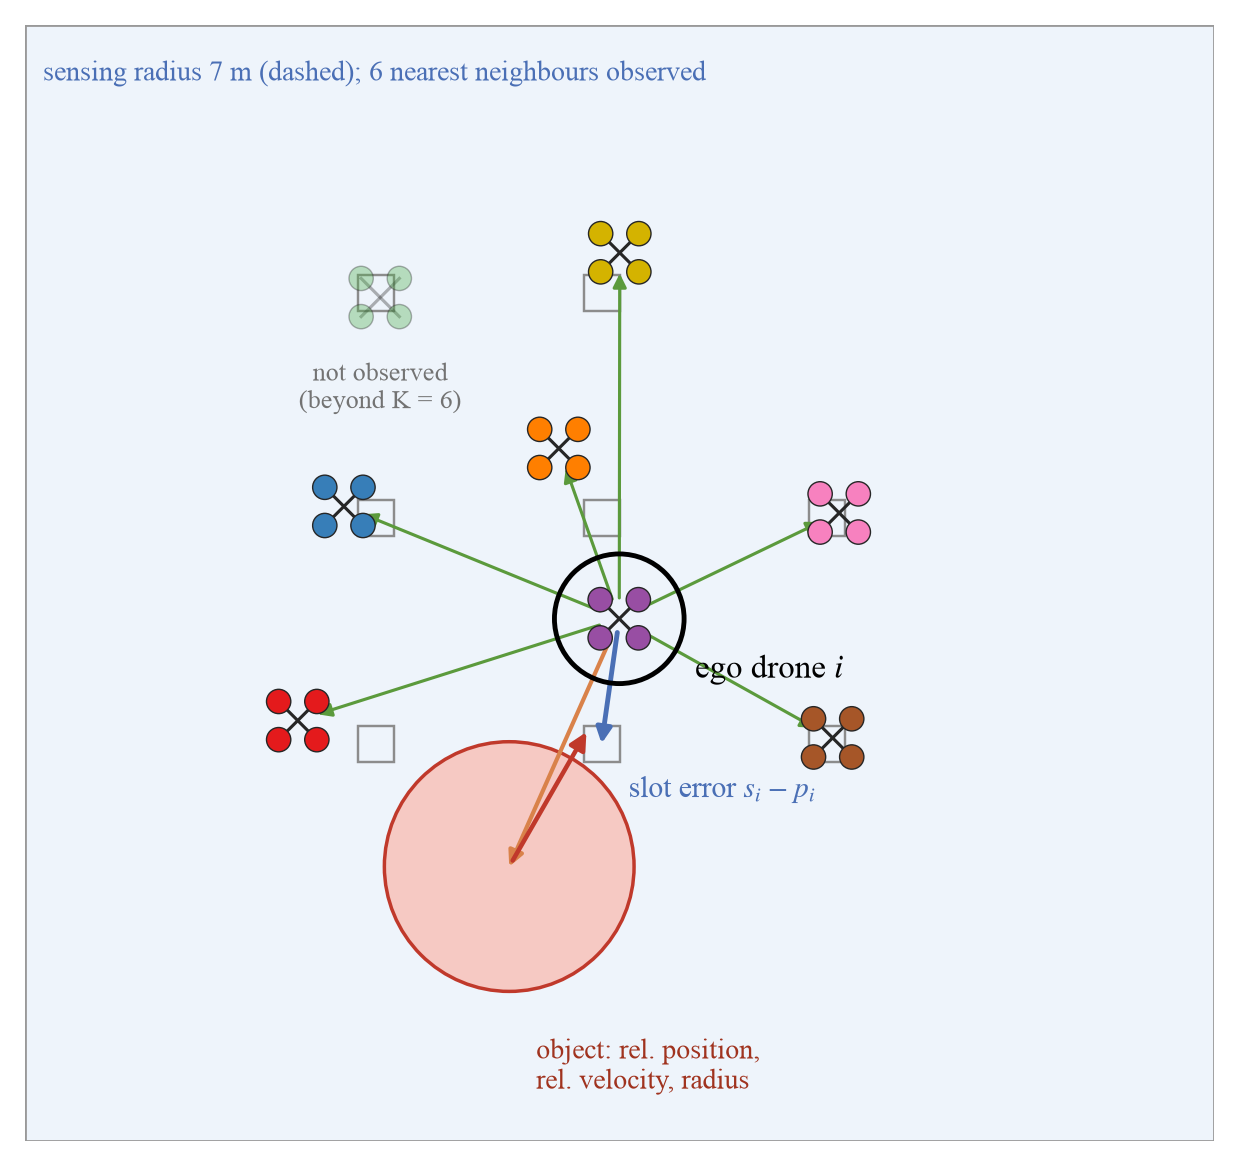
\includegraphics[width=0.48\textwidth]{fig_local_observation}
  \caption[Local observation of one drone]{Local observation of one drone (ego, circled), drawn from a recorded
  simulation state. Green arrows: relative positions of the six nearest neighbours (the seventh drone is not
  observed); orange arrow: relative position of the object, whose velocity is shown in red; blue arrow: slot
  error $s_i - p_i$ to the assigned slot (square).}
  \label{fig:observation}
\end{figure}

\begin{table}[htbp]
\centering
\caption{Observation vector of each drone}
\label{tab:obs}
\small
\begin{tabularx}{\textwidth}{@{}lcX@{}}
\toprule
Part & Size & Content\\
\midrule
$o^{\mathrm{self}}_i$ & 17 & slot error $s_i-p_i$ (3), own velocity (3), target velocity (3), previous command (3),
slot offset $\delta_i$ (3), altitude (1), remaining episode fraction (1)\\
$O^{\mathrm{nbr}}_i$ & $6\times8$ & per neighbour: relative position (3), relative velocity (3), radius (1), validity mask (1)\\
$O^{\mathrm{obj}}_i$ & $6\times8$ & per object: relative position (3), relative velocity (3), radius (1), validity mask (1)\\
\bottomrule
\end{tabularx}
\end{table}

\section{Reward Design}
The reward of drone $i$ at each step is a constant survival term minus a bounded cost,
\begin{equation}
  r_{i,t} = \Delta t\,\bigl(1 - C_{i,t}\bigr) \;-\; 100\cdot\mathbb{1}\!\left[\text{drone } i \text{ involved in a failure}\right],
  \label{eq:reward}
\end{equation}
with $\Delta t = 0.05$\,s. With the slot error $e = \lVert p_i - s_i\rVert$ capped at $e_c = \min(e, 5)$, the
cost is
\begin{equation}
\begin{aligned}
  C ={}& C_{\mathrm{slot}}(e_c) + 0.12\min(\lVert v_i - \dot q\rVert, 3)^2 + 6\,[0.45 - g_{\mathrm{nn}}]_+^2 \\
      &+ 3\min\Bigl(\sum_{o}\bigl[1 - g_o\bigr]_+^2,\, 2\Bigr) + 0.005\lVert u_i\rVert^2
      + 0.001\min\Bigl(\tfrac{\lVert \Delta u_i\rVert}{\Delta t}, 20\Bigr)^2,
\end{aligned}
  \label{eq:cost}
\end{equation}
\begin{equation}
  C_{\mathrm{slot}}(e_c) = \begin{cases} e_c^2, & e_c \le 1\,\text{m},\\ 2e_c - 1, & e_c > 1\,\text{m},\end{cases}
  \label{eq:slotcost}
\end{equation}
where $g_{\mathrm{nn}}$ is the surface gap to the nearest drone, $g_o$ the surface gap (in metres) to each active object
and $[x]_+=\max(0,x)$. Table~\ref{tab:reward} explains each term. Because every cost is capped, the per-step
reward is bounded from below; a unit test confirms that even the worst-case discounted return of a surviving
drone is higher than the $-100$ failure penalty, so ending an episode early is never an easy way to avoid the
costs. The failure penalty is assigned only to the drones involved, so that the learning signal identifies the
responsible agent \cite{batra2021decentralized}.

\begin{table}[htbp]
\centering
\caption{Terms of the per-drone cost}
\label{tab:reward}
\small
\begin{tabularx}{\textwidth}{@{}lcX@{}}
\toprule
Term & Weight & Purpose\\
\midrule
Slot tracking $C_{\mathrm{slot}}$ & 1 & quadratic near the slot, linear far away (bounded gradient)\\
Velocity matching & 0.12 & move with the target velocity\\
Drone proximity & 6 & keep more than 0.45\,m surface gap to the nearest drone\\
Object warning zone & 3 & smooth penalty inside 1\,m of an object, capped at two objects\\
Command effort / rate & 0.005 / 0.001 & smooth, economical velocity commands\\
Failure & $-100$ & collision, ground contact or leaving the flight volume\\
\bottomrule
\end{tabularx}
\end{table}

\section{Policy Network}
The policy (Figure~\ref{fig:network}) follows the self/neighbour/obstacle encoder structure of
\cite{batra2021decentralized,huang2024collision}. The self observation is normalised and encoded by a linear
layer with $\tanh$ activation into $e_{\mathrm{self}}\in\mathbb{R}^{128}$. Each neighbour (or object) row $x_j$ is
encoded by a shared two-layer MLP, $h_j = \phi(x_j)\in\mathbb{R}^{128}$, and the set of rows is pooled by
multi-head attention with a learned query $q$ \cite{huang2024collision}:
\begin{equation}
\begin{aligned}
  \hat e &= \operatorname{MHA}\bigl(q,\,H,\,H\bigr) = \bigl[\operatorname{head}_1,\dots,\operatorname{head}_4\bigr]W^O,\\
  \operatorname{head}_k &= \operatorname{softmax}\Bigl(\frac{qW_k^Q\,(HW_k^K)^\top}{\sqrt{d_k}} + M\Bigr) HW_k^V ,
\end{aligned}
  \label{eq:attention}
\end{equation}
where $H = [h_1,\dots,h_6]$ and the mask $M$ removes padded rows. Because the softmax weights are computed per
row, the result is independent of the order of neighbours \cite{batra2021decentralized}. The three
embeddings are concatenated (384 values) and passed through a trunk MLP (384$\to$256$\to$128). The actor head
outputs the mean $\mu_\theta(o_i)$ of a Gaussian with a learnable, state-independent standard deviation
$\sigma$; the action is squashed with $\tanh$:
\begin{equation}
\begin{aligned}
  &x \sim \mathcal{N}\bigl(\mu_\theta(o_i), \operatorname{diag}\sigma^2\bigr),\qquad a_i = \tanh(x),\\
  &\log\pi_\theta(a_i\mid o_i) = \sum_{k=1}^{3}\Bigl[\log\mathcal{N}(x_k) - \log\bigl(1-\tanh^2 x_k\bigr)\Bigr].
\end{aligned}
  \label{eq:tanh}
\end{equation}
The correction term accounts for the change of variables introduced by the $\tanh$ squashing. At deployment the
deterministic action $a_i = \tanh(\mu_\theta(o_i))$ is used. The critic $V_\phi(o_i)$ has a separate encoder
of the same architecture, so value-loss gradients cannot disturb the actor
features. The actor has 284{,}166 and the critic 283{,}905 trainable parameters.

\begin{figure}[htbp]
  \centering
  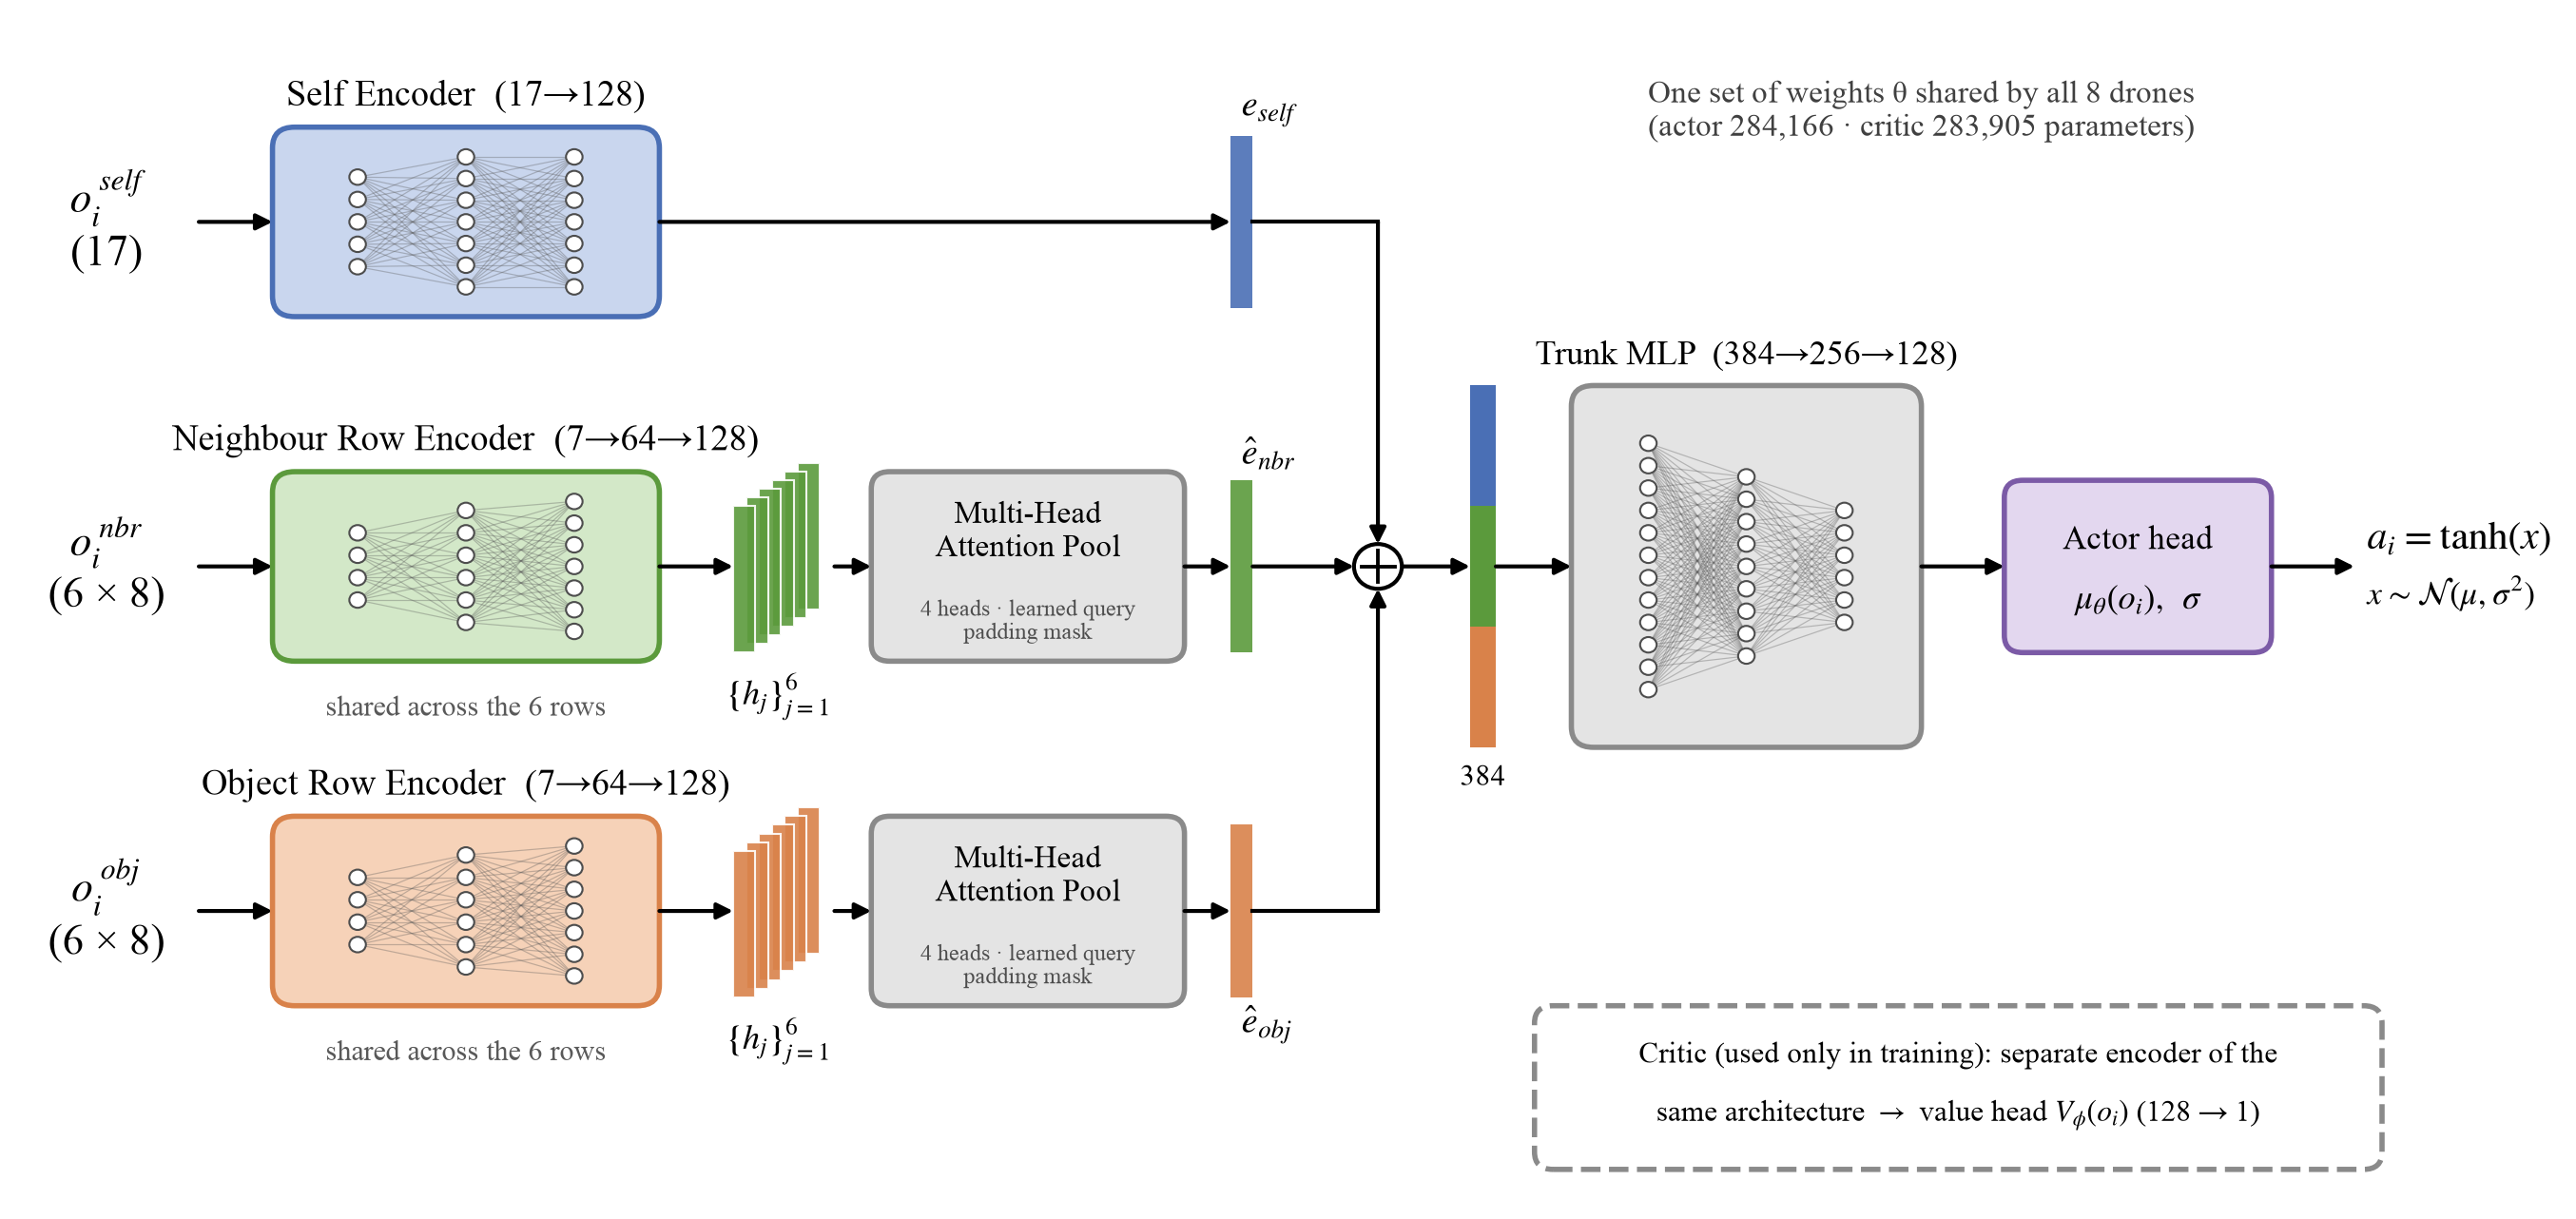
\includegraphics[width=0.9\textwidth]{fig_network_architecture}
  \caption[Architecture of the shared actor network]{Architecture of the shared actor network. Neighbour and
  object rows are encoded by shared MLPs and pooled by masked multi-head attention with a learned query; the
  pooled embeddings are concatenated with the self embedding and mapped to a squashed Gaussian velocity
  action.}
  \label{fig:network}
\end{figure}

\section{Learning Algorithm}
\subsection{Demonstration-guided initialisation}
At the beginning of every curriculum stage the actor is initialised by imitation of a sampling-based
model-predictive expert planner. The planner uses the same local observation; it simulates 86 candidate
velocity commands for 2\,s with the drone's response model, assumes that observed bodies keep their velocity,
and selects the command with the lowest cost for slot tracking and for violating soft (0.6\,m) and hard
(0.25\,m) clearance margins. In round 0 the expert flies with Gaussian action noise ($\sigma = 0.3$) while its
clean actions are recorded (noise-injected demonstrations, often called DART); in rounds 1--3 the current policy flies and the expert
labels every visited state (DAgger \cite{ross2011reduction}). After each round the actor is refit on all data
collected so far by minimising
\begin{equation}
  \mathcal{L}_{\mathrm{BC}}(\theta) = \mathbb{E}_{(o,a^\ast)\sim\mathcal{D}}
  \bigl\lVert \tanh\bigl(\mu_\theta(o)\bigr) - a^\ast \bigr\rVert^2 .
  \label{eq:bc}
\end{equation}

\subsection{Proximal policy optimisation}
The policy is then fine-tuned with PPO \cite{schulman2017proximal}. With the probability ratio
$\rho_t(\theta) = \pi_\theta(a_t\mid o_t)/\pi_{\theta_{\mathrm{old}}}(a_t\mid o_t)$, the clipped surrogate is
\begin{equation}
  \mathcal{L}^{\mathrm{CLIP}}(\theta) = -\,\mathbb{E}_t\Bigl[\min\bigl(\rho_t\hat A_t,\;
  \operatorname{clip}(\rho_t, 1-\epsilon, 1+\epsilon)\,\hat A_t\bigr)\Bigr],\qquad \epsilon = 0.2 .
  \label{eq:ppo}
\end{equation}
Advantages are estimated with GAE \cite{schulman2016gae} ($\gamma = 0.99$, $\lambda = 0.95$):
\begin{equation}
  \delta_t = r_t + \gamma\,(1-d_t)\,V_\phi(o_{t+1}) - V_\phi(o_t), \qquad
  \hat A_t = \delta_t + \gamma\lambda\,(1 - e_t)\,\hat A_{t+1},
  \label{eq:gae}
\end{equation}
where $d_t = 1$ only for a failure and $e_t = 1$ at any episode end; at the 24\,s time limit the value of the
final observation is bootstrapped instead of treated as terminal. The complete loss keeps
a decaying imitation term on the expert data, so that the demonstrated behaviour is retained during fine-tuning:
\begin{equation}
  \mathcal{L}(\theta,\phi) = \mathcal{L}^{\mathrm{CLIP}}(\theta) + 0.5\cdot\tfrac{1}{2}\,\mathbb{E}_t\bigl[(V_\phi(o_t)-\hat R_t)^2\bigr]
  + \beta(f)\,\mathcal{L}_{\mathrm{BC}}(\theta), \qquad \beta(f) = 1.0 - 0.5f,
  \label{eq:loss}
\end{equation}
where $\hat R_t = \hat A_t + V_\phi(o_t)$ and $f\in[0,1]$ is the progress within the stage. Rewards are divided
by a running standard deviation of the discounted return, advantages are normalised, actor and critic
gradients are clipped separately to norm 0.5, the learning rate is annealed linearly to 10\% of its initial
value, and the remaining epochs of an update are skipped when the mean approximate KL divergence of an epoch
exceeds 0.03. Before the first actor update, ten critic-only updates
prepare the value function for the imitation-initialised policy. In the obstacle stages, an episode that ends
in a collision is restored from a snapshot taken a few seconds earlier (at most twice per episode) and continued
with fresh on-policy steps, following the replay idea of \cite{huang2024collision}.

\subsection{Curriculum and model selection}
Training proceeds in three stages of increasing difficulty (a curriculum); each stage keeps the
scenarios of the previous stages and starts from the previous stage's best checkpoint. Every 100{,}000
environment steps the deterministic policy is validated on 10 selection seeds per scenario, and the checkpoint
with the highest selection score
\begin{equation}
  S = \overline{\text{success}} - 0.25\;\overline{\min(\text{RMSE}_{\mathrm{slot}}, 2)} - 0.25\,\bigl(1 - \text{recovered fraction}\bigr)
  \label{eq:score}
\end{equation}
is kept. Training, selection and final testing use disjoint seed ranges (0--999, 5000+, and 100000--100019
respectively), so that the reported test results are never used for tuning.

\section{Evaluation Metrics}
The formation error of an episode is the time-integrated slot RMSE,
\begin{equation}
  \text{RMSE}_{\mathrm{slot}} = \sqrt{\frac{1}{T_e}\sum_{t}\Delta t\,\frac{1}{N}\sum_{i=1}^{N}\lVert p_{i,t} - s_{i,t}\rVert^2 },
  \label{eq:rmse}
\end{equation}
where $T_e$ is the episode duration. A disturbance is \emph{recovered} when, after the object has left the
scene, every drone is simultaneously within 0.35\,m of its own slot and within 0.35\,m/s of the target
velocity for a continuous 1\,s; the recovery time includes this 1\,s confirmation. The minimum surface
clearance over the episode and the fraction of episodes completed without failure complete the evaluation.
